\documentclass[11pt]{article}
\usepackage{amsmath, amssymb, amsthm}
\usepackage[retainorgcmds]{IEEEtrantools}

\usepackage[pdftex]{graphicx}

\usepackage{fancyhdr}

%Format stuff
\pagestyle{fancy}
\headheight 35pt

%Header info
\chead{\Large \textbf{Laplace Transforms}}
\lhead{}
\rhead{}

\newcommand{\Lagr}{\mathcal{L}}

\begin{document}
\section{Definition}
	The Laplace transform $\Lagr[f](s)$ is defined as
	\begin{equation}
		\Lagr[f](s) = \int_0^\infty e^{-st} f(t) dt
	\end{equation}
	
	To apply this transform to an ODE, consider the following property of the transform:
	\begin{equation}
		\Lagr[f'](s) = s\Lagr[f](s) - f(0)
	\end{equation}
	Applied again to make second-order ODE's easier to solve, we get
	\begin{equation}
		\Lagr[f''](s) = s^2\Lagr[f](s) - sf(0) - f'(0)
	\end{equation}
	And generalized to any derivative,
	\begin{equation}
		\Lagr[y^{(n)}](s) = -y^{(n-1)}(0) - sy^{(n-2)}(0) - \ldots -s^{n-2}y(0) + s^n\Lagr[y](s)
	\end{equation}
	
	When a Laplace transform is applied to a differential equation, you can separate terms to get $\Lagr[y](s)$ on one side and all the other s-based terms and initial conditions on the other. Partial fraction decomposition will allow you to take the inverse Laplace.
	
	\begin{figure}[htb]
		\centering
		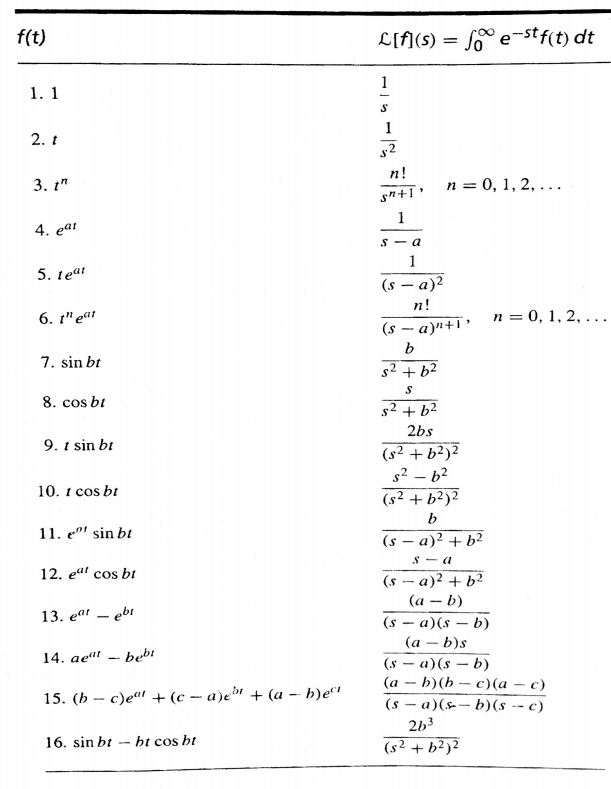
\includegraphics[width=\textwidth]{laplace.png}
	\end{figure}
	
\section{Convolution}
	The convolution of two functions $f$ and $g$ is defined as
	\begin{equation}
		f \ast g(t) = \int_0^t f(u)g(t-u)du
	\end{equation}
	If $f$ and $g$ are integrable on $0 \leq u \leq t$ for every positive $t$, then $f\ast g$ and $g \ast f$ both exist and are equal. Furthermore, if $\Lagr[|f|](s)$ and $\Lagr[|g|](s)$ are both finite, then 
	\begin{equation}
		\Lagr[f\ast g](s) = \Lagr[f](s) \cdot \Lagr[g](s)
	\end{equation}
	
	\begin{figure}[htb]
		\centering
		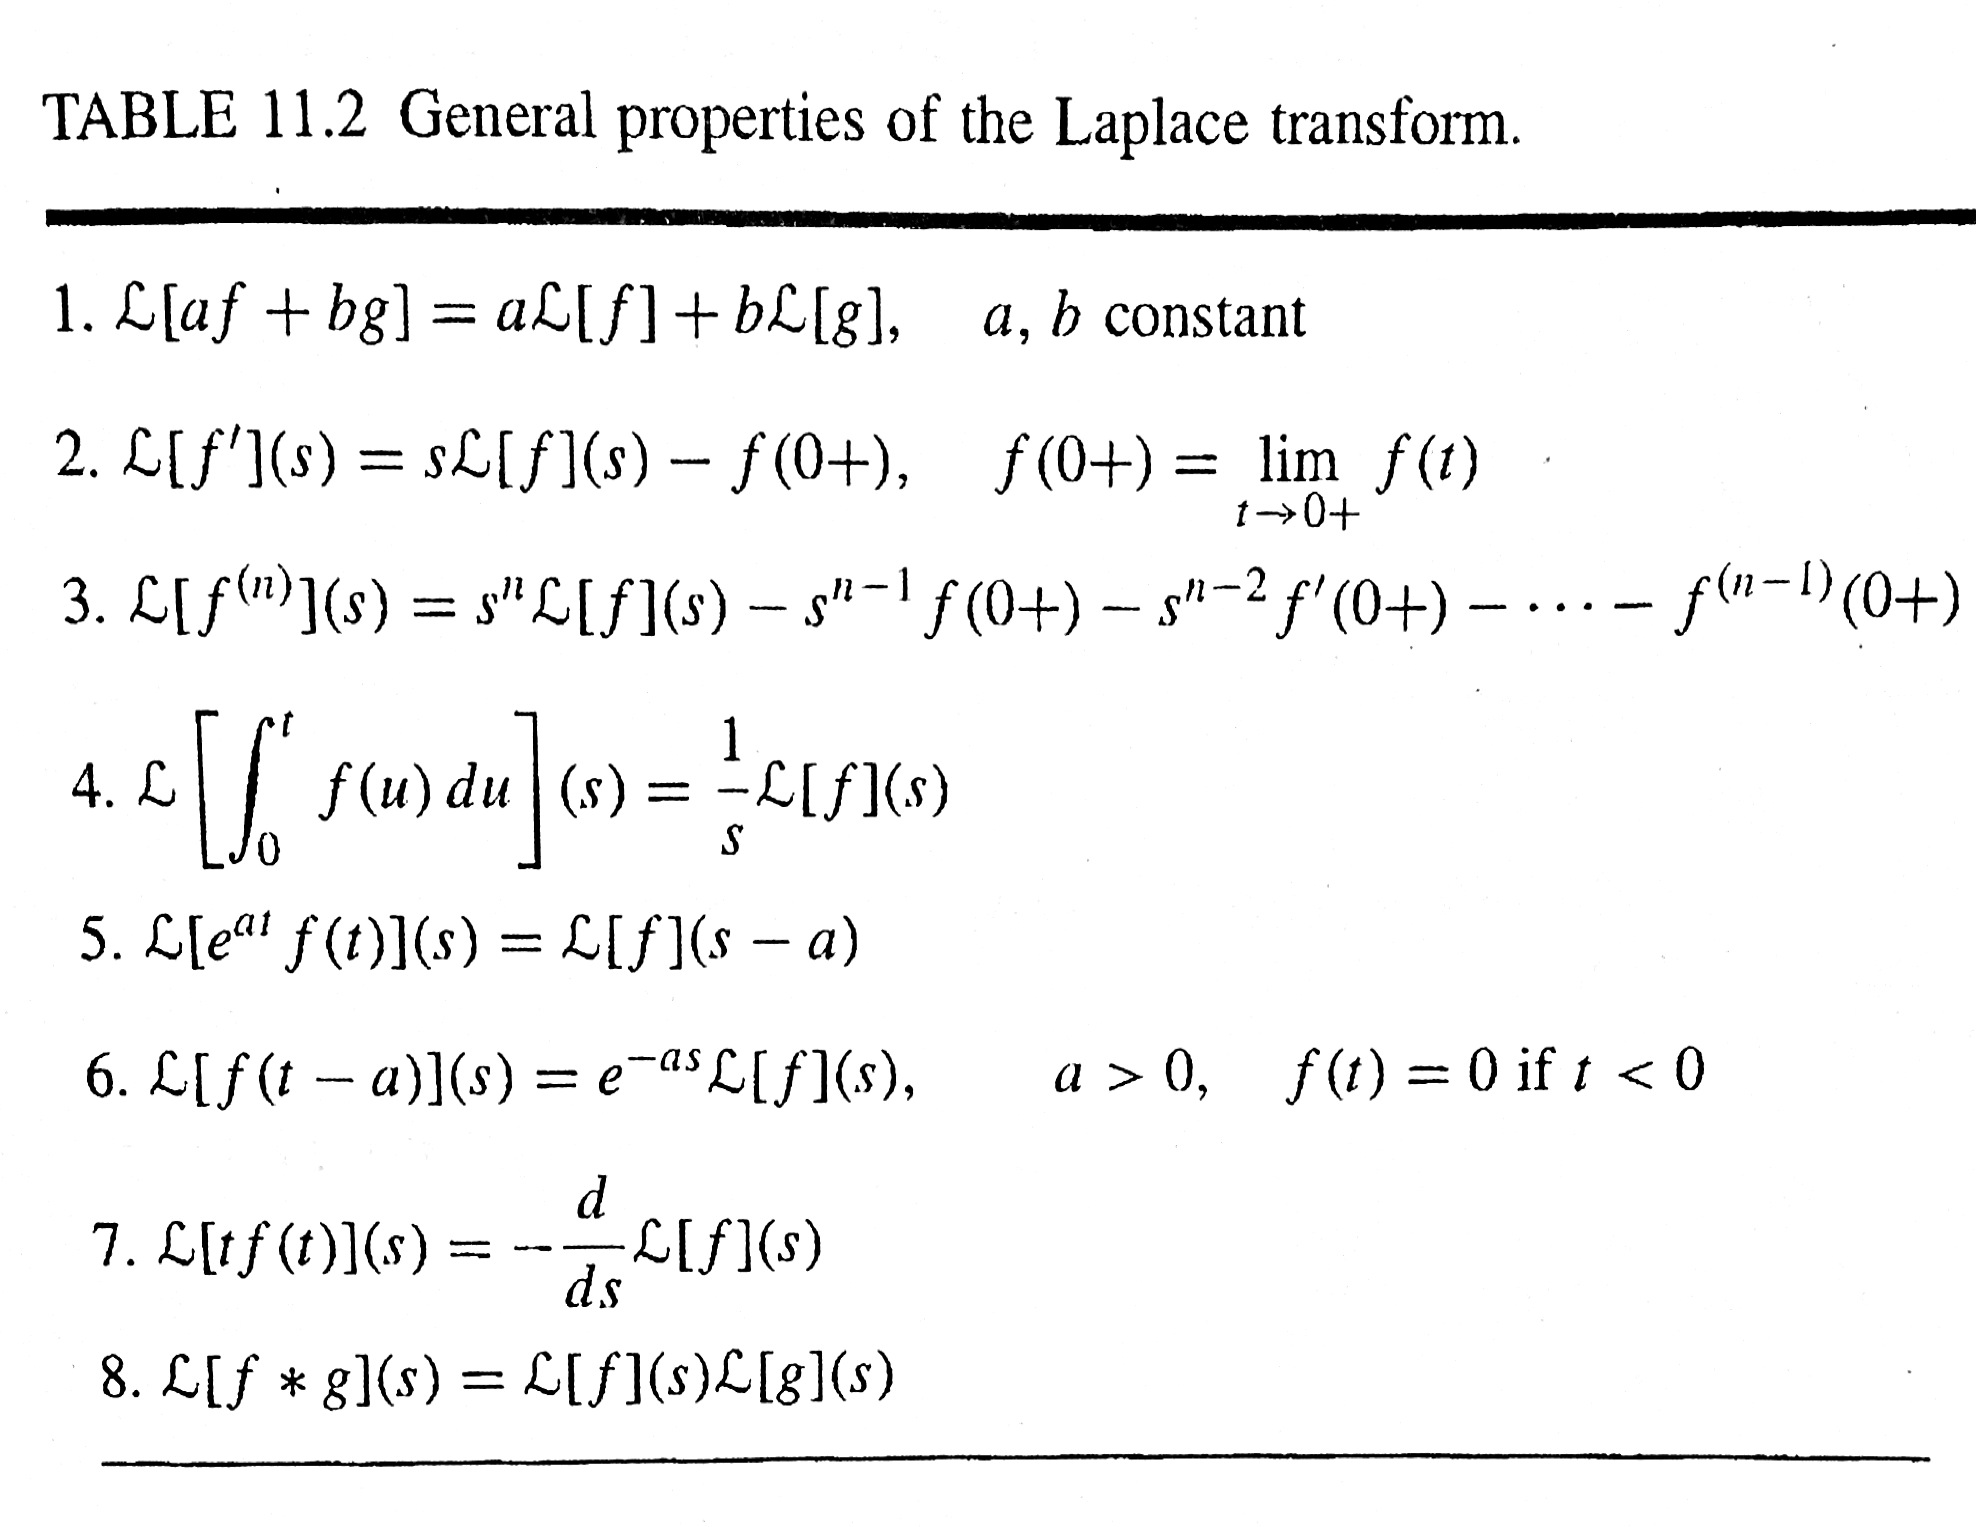
\includegraphics[width=\textwidth]{laplaceprop.jpg}
	\end{figure}

%	\begin{center}
%	\begin{tikzpicture}
%		[scale=3,line cap=round,
%		%Styles
%		axes/.style=,
%		important line/.style={very thick},
%		information text/.style={rounded corners,fill=red!10,inner sep=1ex},
%		dot/.style={circle,inner sep=1pt,fill,label={#1},name=#1}			
%		]
%		
%		%Colors
%		\colorlet{anglecolor}{green!50!black}	%angle arcs/lines
%		
%		%The graphic
%	\end{tikzpicture}
%	\end{center}

%	\begin{figure}[htb]
%		\centering
%		\includegraphics[width=0.8\textwidth]{filename.eps}
%		\caption{Caption.}
%		\label{fig:figure}
%	\end{figure}

%		\def\enotesize{\normalsize}
%		\theendnotes
\end{document}